\documentclass[Thesis.tex]{subfiles}
\begin{document}

\chapter{A variational principle for discrete Tschebyshev nets}

Introduction...

\section{Variational principle}

Let $M=(V,E,F)$ be a quad-mesh. The vertices of $M$ are denoted by $v_i \in V$, the edges
are $e_{\mathrm{\it{ij}}} \in E$, and the quadrilaterals are denoted by $f_{\mathrm{\it{ijkm}}} \in F$.
\section{Energies}
We use a linear combination of energies to enforce desired properties on the optimised mesh.
Our energy consists of three parts.
\begin{equation}
	E(M) =	\lambda_1 E_{\textrm{\scriptsize{ref}}} + 
		\lambda_2 E_{\textrm{\scriptsize{len}}} +
		\lambda_3 E_{\textrm{\scriptsize{cur}}}
	\label{eq:energy_combination}
\end{equation}
The energy $E_{\textrm{\scriptsize{ref}}}$ penalises the distance of vertices from a
reference surface. This surface can be anything that gives a distance function, e.g., a
triangulated surface or a \textsc{Nurbs}-surface. The energy and its gradient are given 
by
\begin{eqnarray*}
	E_{\textrm{\scriptsize{ref}}}(M) &=& 
	\sum_{v_i \in V}\left<v_i - cp_i, v_i - cp_i\right> \\
	\frac{\partial E_\textrm{\scriptsize{ref}}}{\partial v_i} &=&
	2\left(v_i - cp_i\right)
	\label{eq:energy_reference}
\end{eqnarray*}
Here $v_i$ is a vertex of the optimised quad-mesh and $cp_i$ a closest point on the reference
surface measured from vertex $v_i$. The functional $E_{\textrm{\scriptsize{len}}}$ measures
edge length deviation from a given reference length $L$. Its derivative and energy is given as
\begin{eqnarray*}
	E_{\textrm{\scriptsize{len}}}(M) &=& 
	\sum_{e_{\mathrm{\it{ij}}} \in E} \left(\Vert v_i - v_j \Vert - L\right)^2\\
	\frac{\partial E_\textrm{\scriptsize{len}}}{\partial v_i} &=& 
	\sum_{e_{\mathrm{\it{ij}}} \in \textrm{\scriptsize{star}}(v_i)}
	\left(2 - \frac{2L}{\Vert v_i - v_k \Vert}\right)\left(v_i - v_k \right)
\end{eqnarray*}
The sum in the derivative is taken over all edges incident to vertex $v_i$, called the 
edge-star of vertex $v_i$. The third energy is a fairing term that penalises a notion of
curvature of curves on the surface. As we only deal with quad-meshes with $\mathbb Z^2$ combinatorics every interor vertex has four adjacent edges. The energy $E_{\textrm{\scriptsize{cur}}}$ and its gradient is defined as:
\begin{eqnarray*}
	E_{\textrm{\scriptsize{cur}}}(M) &=& \sum_{v_i\in V} \left(\pi - \angle(e_{\mathrm{\it{i1}}}, e_{\mathrm{\it{i3}}}) \right)^2 
	+ \left(\pi - \angle(e_{\mathrm{\it{i2}}}, e_{\mathrm{\it{i4}}}) \right)^2 \\
	\frac{\partial}{\partial v_j}\angle(e_{\mathrm{\it{ij}}},e_{\mathrm{\it{ik}}}) &=& 
	\frac{-1}{\left\Vert e_{\mathrm{\it{ij}}}\right\Vert}\left(e_{\mathrm{\it{ik}}}-e_{\mathrm{\it{ij}}}\frac{\left<e_{\mathrm{\it{ik}}},e_{\mathrm{\it{ij}}}\right>}{\left<e_{\mathrm{\it{ij}}},e_{\mathrm{\it{ij}}}\right>}\right)
	\left\Vert e_{\mathrm{\it{ik}}}-e_{\mathrm{\it{ij}}}\frac{\left<e_{\mathrm{\it{ik}}},e_{\mathrm{\it{ij}}}\right>}		
	{\left<e_{\mathrm{\it{ij}}},e_{\mathrm{\it{ij}}}\right>} \right\Vert^{-1} \\
	\frac{\partial}{\partial v_i}\angle(e_{\mathrm{\it{ij}}},e_{\mathrm{\it{ik}}}) &=& 
	- \left(\frac{\partial}{\partial v_j}\angle(e_{\mathrm{\it{ij}}},e_{\mathrm{\it{ik}}}) + 
	\frac{\partial}{\partial v_k}\angle(e_{\mathrm{\it{ij}}},e_{\mathrm{\it{ik}}})\right)
\end{eqnarray*}
Here and $e_{\mathrm{\it{i1}}}$, $e_{\mathrm{\it{i2}}}$, $e_{\mathrm{\it{i3}}}$, and $e_{\mathrm{\it{i4}}}$ are the adjacent edges of $v_i$ in cyclic order. An edge $e_{\mathrm{\it{ij}}}$ is also used in the role of a vector pointing from vertex $v_i$ to vertex $v_j$. $\angle(e_{\mathrm{\it{ij}}},e_{\mathrm{\it{ik}}})$ is the angle spaned by the vectors $e_{\mathrm{\it{ij}}}$ and $e_{\mathrm{\it{ik}}}$  From the angle derivatives with respect to the vertices the gradient can be computed efficiently.

\begin{figure}[ht]
\centering
\resizebox{\textwidth}{!}{
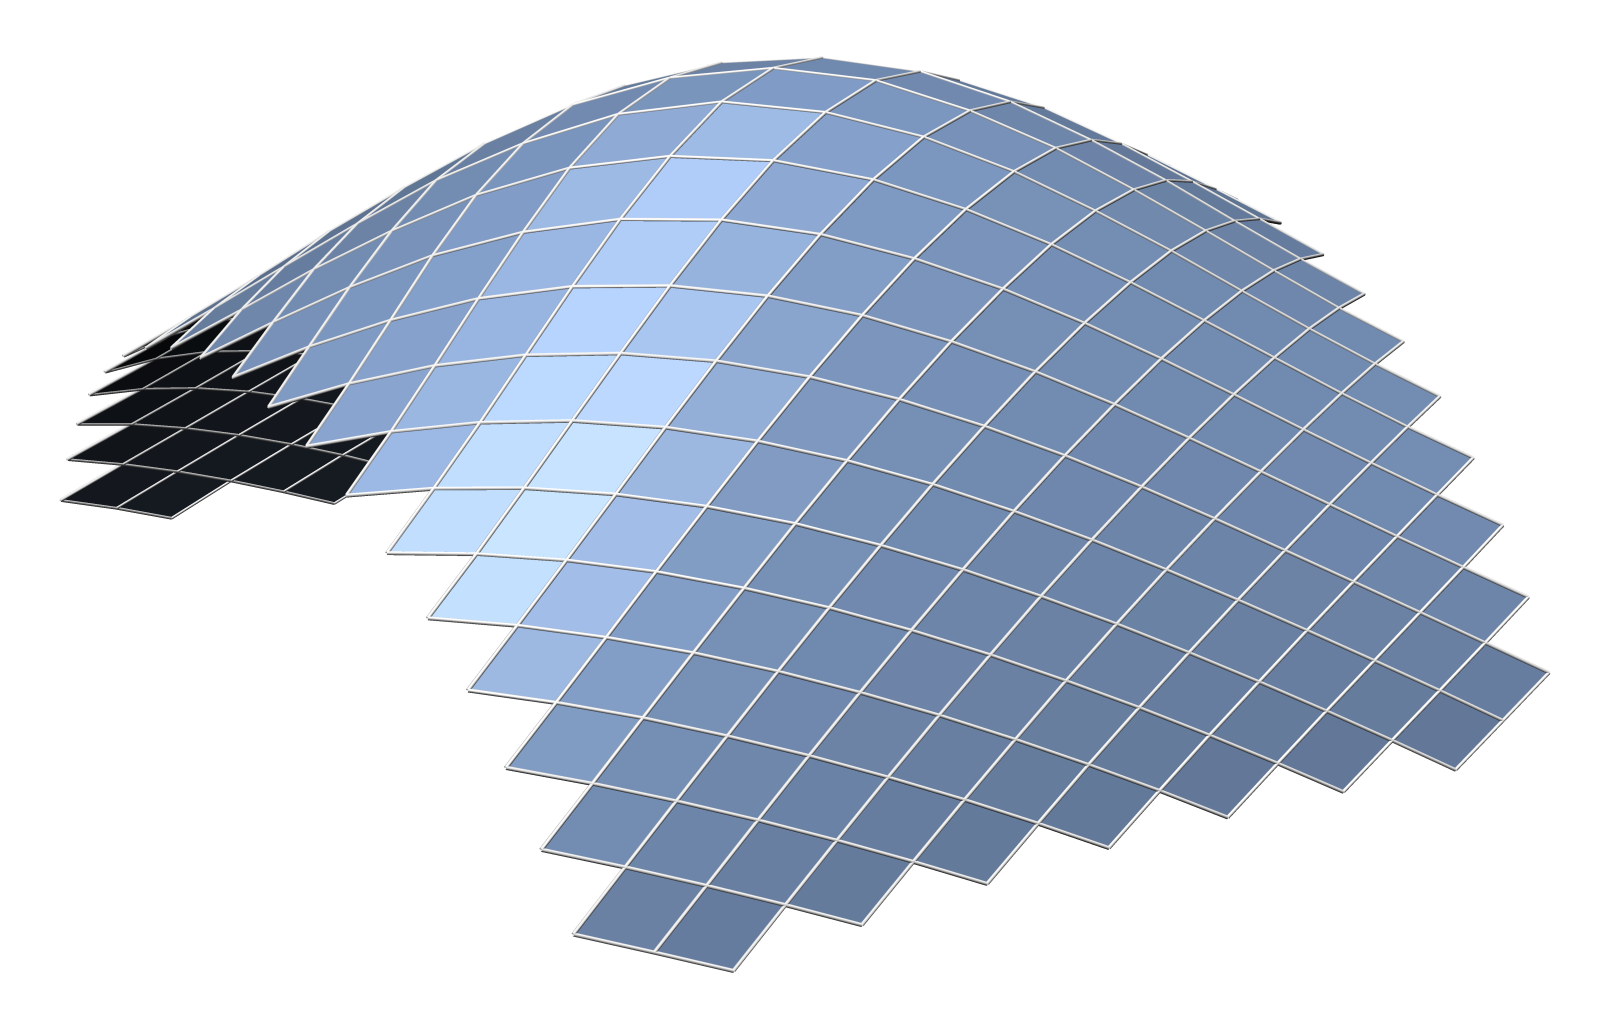
\includegraphics[width=0.33\linewidth]{image/tscheby/init60_mesh.png}
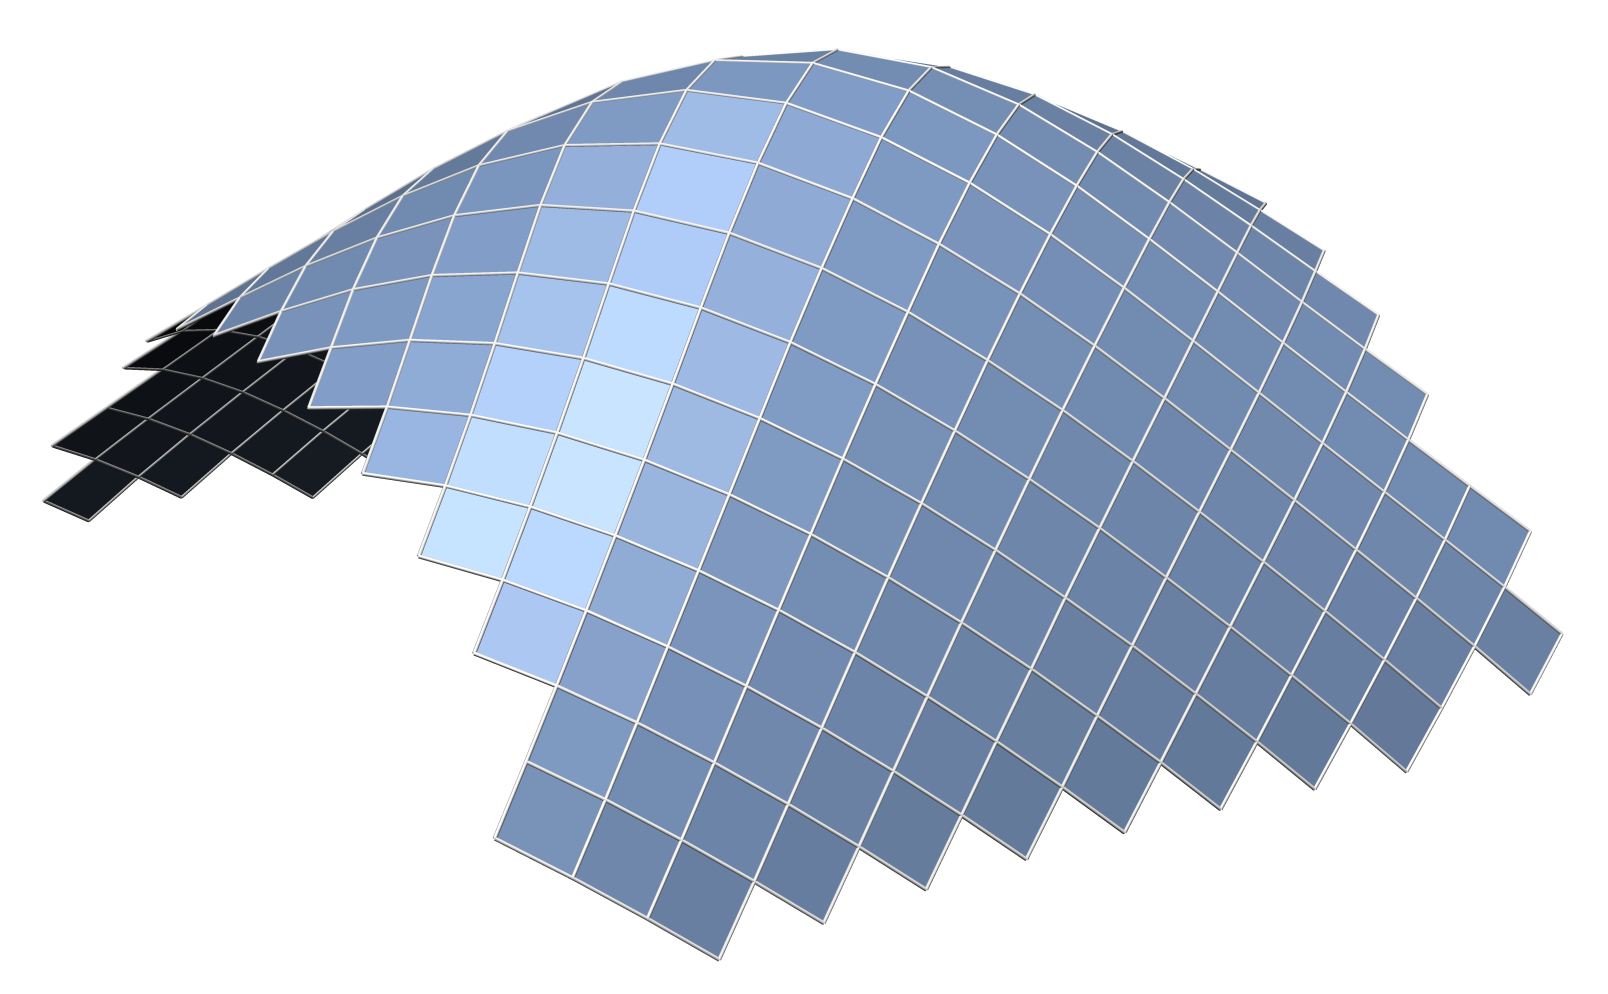
\includegraphics[width=0.33\linewidth]{image/tscheby/init90_mesh.png}
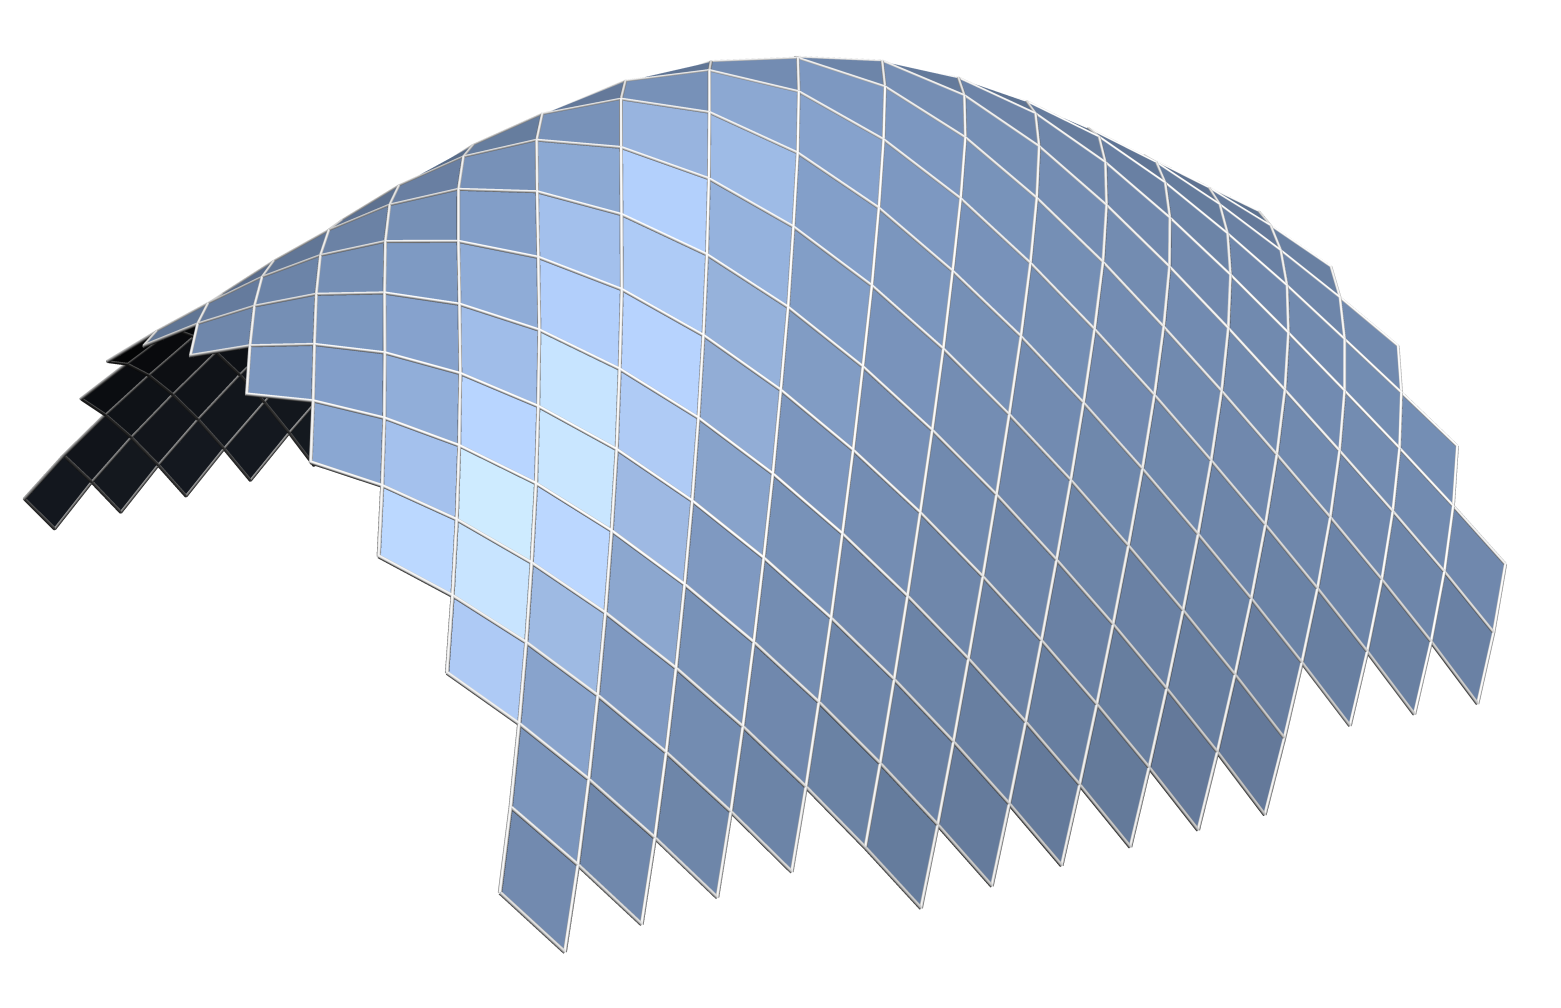
\includegraphics[width=0.33\linewidth]{image/tscheby/init120_mesh.png}
}
\caption{Different initialization shear angles for a conformal remesh. $30^\circ$ left, $0^\circ$ middle, and $-30^\circ$ right.}
\label{fig:initial_grids}
\end{figure}
\section{Initialization and parameters}
The energy $E(M)$ is in general non-convex. That means there can be many local optima, and the solution found by some gradient descent depends on the initialisation. We propose to use a conformal remesh of the reference surface as initialization. The conformality of the parameterisation gives us control over the angles between edges of the quadrilaterals. We can introduce shear to the parameterisation and modify this angle globally. By this we start with meshes that have almost constant edge angle (see Fig.~\ref{fig:initial_grids}).

\section{Implementation}
We use the conformal mapping algorithm by \cite{Springborn2008} to create the
initial mesh. To minimize the energy $E(M)$ we use the non-linear optimization package
PETSc/TAO \cite{petsc-web-page,tao-user-ref} and its java binding 
\cite{jpetsctao-web-page}. We have made good experiences with normalising the
 energies to have gradient length one before optimization. Then we start with all
$\lambda$s equal to one and modify them on the way if needed. If one encounters
degenerate configurations during optimization one can drop the length energy term for 
a few iterations.

\subfilebibliography
\end{document}

%%% Local Variables:
%%% TeX-master: "Thesis.tex"
%%% End: